\section{The Latitude Blockchain}\label{sec:design}

In this section, we present a high-level design of the Latitude blockchain. The full-version of this whitepaper shall
contain a very detailed design of each component. We start with an overview of the key design principles that will guide
the rest of the design for the Latitude Blockchain. Its important to note here that for implementation purposes, it
might be possible to use an existing core blockchain for the underlying functionalities and build Latitude as a layer on
top. We shall make these determinations in the full-version of the whitepaper.

\subsection{Design overview}

The purpose of the Latitude blockchain is to become the best platform in the world for decentralized applications for
the Transportation Industry. Specifically, this boils down to constructs in the blockchain that can handle spatial,
mapping, traffic, driving data including data relating to other modalities of transport (bike sharing, walking, even air
routes later on). Figure XXX presents the architecture of the Latitude blockchain in terms of the core technological
innovations that will be built into it.

\begin{figure}[t]
    \centering
    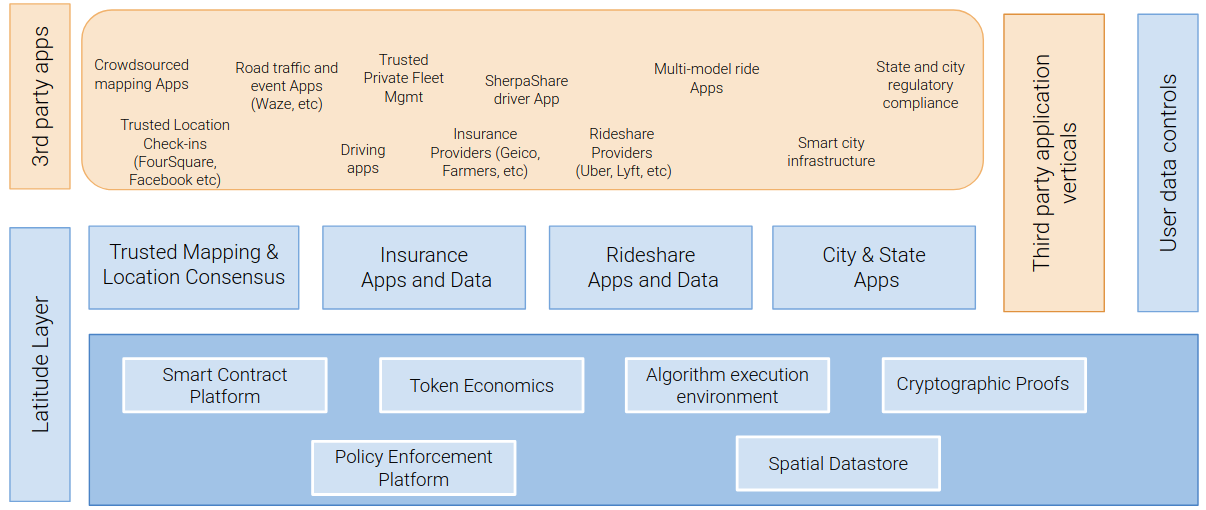
\includegraphics[width=0.90\textwidth]{latarch.png}
  \caption{Architecture of the Latitude Blockchain and associated platform ecosystem.}
    \label{fig:lat-arch}
\end{figure}

One of the central aspects of the Latitude blockchain is a geo-spatial datastore that fundamentally understands various
datatypes that are specific to transportation data. This datastore can use existing GIS databases that allow
de-centralized storage and access. The types of data include (i) georaphic data such as location (latitude, longitude),
(ii) mapping data such as roads, terrain, addresses, etc, (iii) sensor data such as driving data, driver score, miles
driven, route information, etc, (iv) multi-modal transport data such as biking, walking and other means of transport.
Each of these data types have very special characteristics which the underlying datastore can be optimized for and allow
for programming using what we call the {\em Latitude Smart Contract} framework. 

The datastore would include spatial, quad-tree or an R-tree based indexes for efficient querying and other operations that
most Geographic Information Systems (GIS) would support in a centralized manner today. It would also include functions
to compute heatmaps, driving maps and statistics such as Traffic predictions including real-time analytics. Depending on
how Latitude evolves, the datastore can include additional functionalities to support the data sharing among autonomous
vehicles since they use most of the similar datatypes mentioned above. The datastore would support circular, rectangular
and other range queries, K-nearest neighbor searches, route optimization algorithms, etc. Figure
\ref{fig:geo_spatial_query} shows some of the queries that such a datastore can support.

\begin{figure}[t]
    \centering
    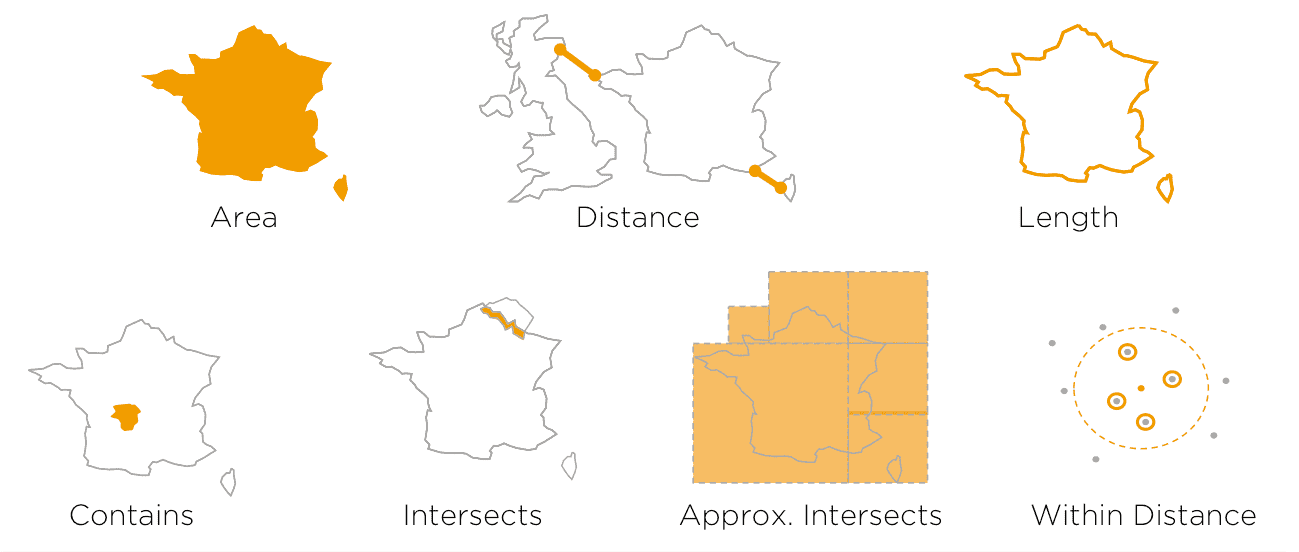
\includegraphics[width=0.90\textwidth]{geospatial_query.png}
  \caption{Examples of Geo-spatial queries that a spatial datastructure can support on the Latitude blockchain.}
    \label{fig:geo_spatial_query}
\end{figure}


Datastore
 - Optimized for Geographic, Geo-spatial data.
 - Location, Mapping data and computation.
 - Ability to Store, index, query and build smart contracts optimized for such data.
 - Support for various spatial indexes.
 - Location heatmaps.
 - Indexing road and driving data.
 - Primitives for storing driving data for autonomous vehicles

\noindent
{\textsf Strong crytographic foundation:}
Standard data encryption techniques allow for security guarantees in Latitude. Anonymity guarantees are provided using
privacy-preserving set operations such as given in \cite{kissner_set}, with suitable modifications to
anonymize spatial data which have user-location considerations \cite{divanis_kanon,xu_loc_anon}.
Cryptographic primitives for:
 - Security and privacy of data.
 - Anonymity guarantees using cryptographic set operations.
 - Enforcement of privacy when sharing data.
 - Sharing of “computation” instead of data when possible.
 - For eg: Sharing of DriverScore using a vetted algorithm.
 - Sharing proximity to a landmark instead of lat/lng.
 - Ability to find bad actors.
 - Detect privacy, anonymity and security violations.

\noindent
{\textsf Latitude Smart contract system:}

Smart contract system for Transportation applications.
 - Ability to convert “policies” such as GDPR into smart contract code.
 - Example, self destruct data after a time period.
 - Sandboxed trusted execution environment:
 - For algorithms:
   - DriverScore, Location heatmaps, Statistics.
   - Enforcing or verifying privacy and other govt policies/regulations.

Cryptographic proofs for applications:
 - Proof of Location. 
 - Proof of ride. 
 - Proof of mapping 
      (road/landmark exists or does not exist).
 - Proof of driver score 
 - Open, trusted, understood driver score computation algorithms.
 - Cryptographic proofs can be shared among entities, safely, securely.

\noindent
\subsection{Cryptoeconomics and Governance:}
Cryto-economics refers to the mechanics of the protocol underlying the blockchain operations which creates incentives
for the various stakeholders. For example, in the Latitude Blockchain it is possible to reward users for sharing their data
for certain purposes. For example, users can be rewarded if they share traffic data or accident information or better
routes. This is similar to the Waze model but creates legitimate rewards for users that have meaningful value outside
the Waze application. For an overview of cryptoeconomics in the blockchain space, please see \cite{sinclair_crypto}.

The core building block of the cryptoeconomics in Latitude is the Latitude Token, or LAT. This will be transacted in
each and every micro-transaction that takes place on the blockchain to create the right incentives, enforce smart
contracts and penalize Byzantine behavior. One of the fundamental design principles behind the protocol for the LAT
token is to create incentives assuming nodes are greedy and are interested in maximizing their gain. We will also build
safeguards against reasonable amount of collusion among nodes to subvert the system. The design is crafted such that the
best way for a node to maximize its revenue would be to participate with full honesty.

Latitude shall employ a Proof of Stake model (delegated or non-delegted) for particpation and core node-level mining. This mechanism has recently
gained popularity among a notable number of blockchains \cite{dpos_steemit}. This also allows for deposit slashing as a
technique to tackle Byzantine behavior. Latitude will employ techniques such as Minimal Slashing \cite{buterin_slashing}
for Byzantine fault tolerance and safety under distributed asynchronous operation.


Governance refers to a decentralized manner in which decisions are made using a consensus mechanism on the blockchain.
Decisions include basic constructs whether a node can join or leave the network. Or it can include key decisions on
whether an upgrade should be mandated on every node, a given participant such as a data provider should be penalized. It
could also include issues where humans get involved, such as when a user complains of a loss of privacy or a breach in
contract.

Recently blockchains have been moving towards governance using a small set of participants, such as trusted miners in
the case of Stellar and Ripple \cite{stellar_gateways}. The EOS blockchain uses a similar concept of a core set of block
producers. For discussion around Governance in Ethereum, refer to \cite{buterin_gov}.

 - Crypto-incentives for honest operation.
 - Penalties for malicious intent.
 - Governance based on consensus and roles using a council.
 - Council members elected using voting, stake and established trust.
 - Some council members can have restricted access.
 - Eg: US govt can have voting rights on US data/users, etc.

User incentives:
 - Users have full control over their data and computation.
 - Users can issue or request proofs to carry over to other applications.
 - User’s have incentive to share data, participate in improving the common denominator.
 - Malicious intent, Byzantine behavior.
   - Can be detected using a combination of consensus and incentives.
   - Best interest of users to act honestly by design.


\noindent
{\textsf Performance considerations:}
Performance:
- Transaction speed. Data throughput. Storage capabilities.
